\documentclass[PhD-Yoann-Dupont.tex]{subfiles}
\begin{document}

Je prévois de poursuivre mes développements sur SEM, afin de le rendre plus complet, autant au niveau des tâches effectuées que du nombre de langues traitées ou des formats gérés. Un format intéressant pour SEM à traiter est le HTML, dont une première implémentation est faite qui doit encore être finalisée pour être rendue disponible. Traiter ce type de fichier permettait de travailler sur des pages web afin d'annoter des documents libres comme ceux de Wikipedia et de ses projets frères, comme wikinews, wikisource et wikibooks. Des exemples sont disponibles dans les figures \ref{fig:sem-wikisource} pour le livre "À l'ombre des jeunes filles en fleurs" de Marcel Proust, disponible sur wikisource\footnote{url du livre : \url{https://fr.wikisource.org/wiki/À_l'ombre_des_jeunes_filles_en_fleurs}} et \ref{fig:sem-wikipedia} pour Wikipédia\footnote{url de l'article : \url{https://fr.wikipedia.org/wiki/Wikipédia}}. Les procédures d'\textit{active learning}, décrites dans la section \ref{subsec:perspectives-active-learning}, afin d'annoter plus rapidement un maximum de livres afin de fournir un grand volume de données annotées. Un projet dans lequel SEM pourrait être utilisé est le "Free French Treebank" de \citet{hernandez2013construction}, dont le but est de fournir un corpus du français annoté et en perpétuelle évolution. Ce dernier comprend environ 2,5 millions de tokens pour environ 87500 phrases. Pour l'instant, ce dernier n'est annoté qu'en POS, l'ajout des entités nommées serait donc intéressant pour le projet, un problème du French Treebank en entités nommées étant sa taille plutôt faible. Ici aussi, les procédures d'\textit{active learning} permettraient de fournir des annotations de référence à un coût humain moins important. Ces annotations fournies seraient triées par type de texte (journalistique, littéraire, etc.) et permettraient d'évaluer la robustesse des annotateurs sur les différents types de texte.

\begin{figure}[ht!]
\centering
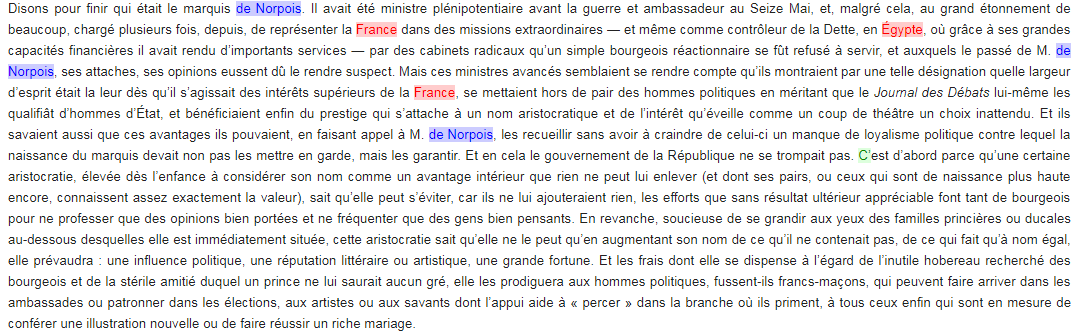
\includegraphics[scale=0.5]{images/SEM/futur-sem-wikisource}
\caption{extrait de "À l'ombre des jeunes filles en fleurs" de Marcel Proust, annotée par SEM. Livre disponible sur wikisource.}
\label{fig:sem-wikisource}
\end{figure}

\begin{figure}[ht!]
\centering
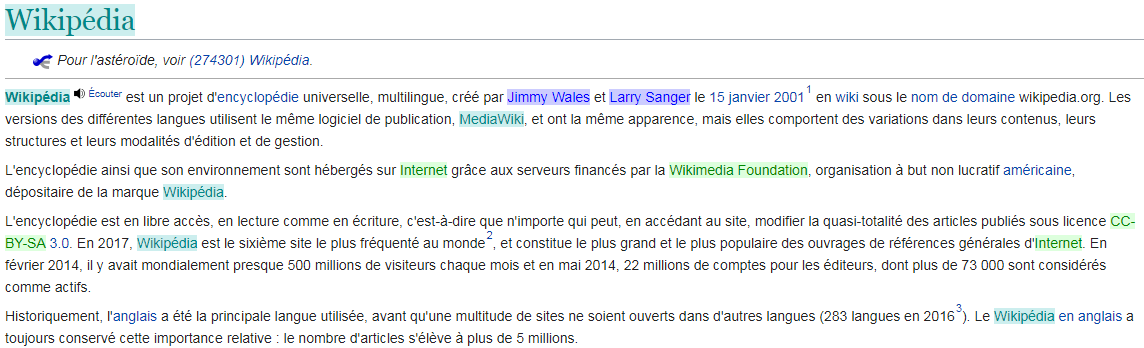
\includegraphics[scale=0.5]{images/SEM/futur-sem-Wikipedia}
\caption{extrait de l'article "Wikipédia" de Wikipédia français, annoté par SEM.}
\label{fig:sem-wikipedia}
\end{figure}

Un autre ajout à SEM serait l'intégration des dépendances syntaxiques. En effet, ces dernières sont utiles pour annoter les entités nommées car elles permettent de capturer des patrons linguistiques \citep{nguyen2016j,jie2017efficient}. Nous prévoyons d'utiliser des traits basés sur les dépendances syntaxiques comme ceux définies par \citet{mintz2009distant}, utilisés dans le cadre de l'extraction de relations. Dans ce cadre, ces dépendances sont généralement utilisées en se référant à un couple d'entités. Dans le cas où ces entités doivent être identifiées, il n'est pas possible de les utiliser à l'identique. Nous pouvons cependant reconstituer des chemins de dépendances. Ces derniers peuvent être de taille fixe, ils seraient alors un contexte gauche et droit comme on le fait classiquement pour les tokens. Il est également possible de recréer le chemin jusqu'à des tokens ayant une catégorie syntaxique intéressante, comme par exemple les verbes et les noms. Si un chemin en dépendances est retracé jusqu'à un verbe, il est possible d'utiliser la classification des verbes de \citet{dubois1997synonymie}, qui permetrait d'obtenir une généralisation de l'information intéressante comme le fait qu'un verbe soit un verbe de parole ou d'action.

Outre les extensions tenant de l'ingénirie, je compte également enrichir SEM des travaux effectués durant cette thèse, principalement l'extraction d'affixes fréquents et la structuration des entités nommées. SEM dispose déjà des répertoires décrits dans la section \ref{subsec:ontology-integration}, mais tous les travaux présentés dans cette thèse n'ont pas encore eu la possibilité d'être intégrés à SEM.

Comme nous l'avons vu précédemment, il existe des problèmes liés aux corpus annotés en entités nommées, comme le manque de calcul inter-annotateurs et l'annotation faite depuis zéro qui s'avère généralement coûteuse en temps. Dans la prochaine perspective, nous explorons une piste afin d'améliorer ces aspects.

\end{document}